%%
%% Automatically generated file from DocOnce source
%% (https://github.com/hplgit/doconce/)
%%

% #define PREAMBLE

% #ifdef PREAMBLE
%-------------------- begin preamble ----------------------

\documentclass[%
oneside,                 % oneside: electronic viewing, twoside: printing
final,                   % draft: marks overfull hboxes, figures with paths
10pt]{article}

\listfiles               % print all files needed to compile this document

\usepackage{relsize,makeidx,color,setspace,amsmath,amsfonts,amssymb}
\usepackage[table]{xcolor}
\usepackage{bm,microtype}

\usepackage[pdftex]{graphicx}

\usepackage{fancybox}  % make sure fancybox is loaded before fancyvrb
%\setlength{\fboxsep}{8pt}  % may clash with need in pre/cod envirs

% Movies are handled by the href package
\newenvironment{doconce:movie}{}{}
\newcounter{doconce:movie:counter}


% Packages for typesetting blocks of computer code
\usepackage{fancyvrb,framed,moreverb}

% Define colors
\definecolor{orange}{cmyk}{0,0.4,0.8,0.2}
\definecolor{tucorange}{rgb}{1.0,0.64,0}
\definecolor{darkorange}{rgb}{.71,0.21,0.01}
\definecolor{darkgreen}{rgb}{.12,.54,.11}
\definecolor{myteal}{rgb}{.26, .44, .56}
\definecolor{gray}{gray}{0.45}
\definecolor{mediumgray}{gray}{.8}
\definecolor{lightgray}{gray}{.95}
\definecolor{brown}{rgb}{0.54,0.27,0.07}
\definecolor{purple}{rgb}{0.5,0.0,0.5}
\definecolor{darkgray}{gray}{0.25}
\definecolor{darkblue}{rgb}{0,0.08,0.45}
\definecolor{darkblue2}{rgb}{0,0,0.8}
\definecolor{lightred}{rgb}{1.0,0.39,0.28}
\definecolor{lightgreen}{rgb}{0.48,0.99,0.0}
\definecolor{lightblue}{rgb}{0.53,0.81,0.92}
\definecolor{lightblue2}{rgb}{0.3,0.3,1.0}
\definecolor{lightpurple}{rgb}{0.87,0.63,0.87}
\definecolor{lightcyan}{rgb}{0.5,1.0,0.83}

\colorlet{comment_green}{green!50!black}
\colorlet{string_red}{red!60!black}
\colorlet{keyword_pink}{magenta!70!black}
\colorlet{indendifier_green}{green!70!white}

% Backgrounds for code
\definecolor{cbg_gray}{rgb}{.95, .95, .95}
\definecolor{bar_gray}{rgb}{.92, .92, .92}

\definecolor{cbg_yellowgray}{rgb}{.95, .95, .85}
\definecolor{bar_yellowgray}{rgb}{.95, .95, .65}

\colorlet{cbg_yellow2}{yellow!10}
\colorlet{bar_yellow2}{yellow!20}

\definecolor{cbg_yellow1}{rgb}{.98, .98, 0.8}
\definecolor{bar_yellow1}{rgb}{.98, .98, 0.4}

\definecolor{cbg_red1}{rgb}{1, 0.85, 0.85}
\definecolor{bar_red1}{rgb}{1, 0.75, 0.85}

\definecolor{cbg_blue1}{rgb}{0.87843, 0.95686, 1.0}
\definecolor{bar_blue1}{rgb}{0.7,     0.95686, 1}
%\setlength{\fboxsep}{-1.5mm}  % do not change since !bbox needs it positive!

%% Background for code blocks (parameter is color name)

%% pro/cod_vpad: gives some vertical padding before and after the text
%% (but has more simplistic code than _cod/pro_tight+cod/pro).
%% pro/cod_vpad can be used to enclose Verbatim or lst begin/end for code.
%% pro/cod calls _pro/cod_tight and has very little vertical padding,
%% used to enclose Verbatim and other begin/end for code.
%% (pro/cod is what the ptex2tex program could produce with the
%% Blue/BlueBar definitions in .ptex2tex.cfg.)

\newenvironment{cod_vpad}[1]{
   \def\FrameCommand{\colorbox{#1}}
   \MakeFramed{\FrameRestore}}
   {\endMakeFramed}

\newenvironment{_cod_tight}[1]{
   \def\FrameCommand{\colorbox{#1}}
   \FrameRule0.6pt\MakeFramed {\FrameRestore}\vskip3mm}
   {\vskip0mm\endMakeFramed}

\newenvironment{cod}[1]{
\bgroup\rmfamily
\fboxsep=0mm\relax
\begin{_cod_tight}{#1}
\list{}{\parsep=-2mm\parskip=0mm\topsep=0pt\leftmargin=2mm
\rightmargin=2\leftmargin\leftmargin=4pt\relax}
\item\relax}
{\endlist\end{_cod_tight}\egroup}

%% Background for complete program blocks (parameter 1 is color name
%% for background, parameter 2 is color for left bar)
\newenvironment{pro_vpad}[2]{
   \def\FrameCommand{\color{#2}\vrule width 1mm\normalcolor\colorbox{#1}}
   \MakeFramed{\FrameRestore}}
   {\endMakeFramed}

\newenvironment{_pro_tight}[2]{
   \def\FrameCommand{\color{#2}\vrule width 1mm\normalcolor\colorbox{#1}}
   \FrameRule0.6pt\MakeFramed {\advance\hsize-2mm\FrameRestore}\vskip3mm}
   {\vskip0mm\endMakeFramed}

\newenvironment{pro}[2]{
\bgroup\rmfamily
\fboxsep=0mm\relax
\begin{_pro_tight}{#1}{#2}
\list{}{\parsep=-2mm\parskip=0mm\topsep=0pt\leftmargin=2mm
\rightmargin=2\leftmargin\leftmargin=4pt\relax}
\item\relax}
{\endlist\end{_pro_tight}\egroup}

\usepackage{listingsutf8}

% Common lstlisting parameters
\lstset{
  basicstyle=\small \ttfamily,
  breaklines=false,          % break/wrap lines
  breakatwhitespace=true,    % let linebreaks happen at whitespace
  breakindent=40pt,
  tab=,
  tabsize=4,                 % tab means 4 spaces
  %belowskip=\smallskipamount,  % space between code and text below
  xleftmargin=5pt,           % indentation of code frame
  xrightmargin=5pt,
  framexleftmargin=5pt,      % add frame space to the left of code
  %numbers=left,             % put line numbers on the left
  %stepnumber=2,             % stepnumber=1 numbers each line, =n every n lines
  %framerule=0.4pt           % thickness of frame
  aboveskip=2ex,             % vertical space above code frame
  showstringspaces=false,    % show spaces in strings with an underscore
  showspaces=false,          % show spaces with an underscore
  showtabs=false,
  keepspaces=true,
  columns=fullflexible,      % tighter character kerning, like verb
  escapeinside={||},         % for |\pause| in slides and math in code blocks
  extendedchars=\true,       % allows non-ascii chars, does not work with utf-8
}

% Internally defined styles for lstlisting

\lstdefinestyle{simple}{
commentstyle={},
}

% end of custom lstdefinestyles

\usepackage[T1]{fontenc}
%\usepackage[latin1]{inputenc}
\usepackage{ucs}
\usepackage[utf8x]{inputenc}

\usepackage{lmodern}         % Latin Modern fonts derived from Computer Modern

% Hyperlinks in PDF:
\definecolor{linkcolor}{rgb}{0,0,0.4}
\usepackage{hyperref}
\hypersetup{
    breaklinks=true,
    colorlinks=true,
    linkcolor=linkcolor,
    urlcolor=linkcolor,
    citecolor=black,
    filecolor=black,
    %filecolor=blue,
    pdfmenubar=true,
    pdftoolbar=true,
    bookmarksdepth=3   % Uncomment (and tweak) for PDF bookmarks with more levels than the TOC
    }
%\hyperbaseurl{}   % hyperlinks are relative to this root

\setcounter{tocdepth}{2}  % number chapter, section, subsection

% Tricks for having figures close to where they are defined:
% 1. define less restrictive rules for where to put figures
\setcounter{topnumber}{2}
\setcounter{bottomnumber}{2}
\setcounter{totalnumber}{4}
\renewcommand{\topfraction}{0.95}
\renewcommand{\bottomfraction}{0.95}
\renewcommand{\textfraction}{0}
\renewcommand{\floatpagefraction}{0.75}
% floatpagefraction must always be less than topfraction!
% 2. ensure all figures are flushed before next section
\usepackage[section]{placeins}
% 3. enable begin{figure}[H] (often leads to ugly pagebreaks)
%\usepackage{float}\restylefloat{figure}

% prevent orhpans and widows
\clubpenalty = 10000
\widowpenalty = 10000

\newenvironment{doconceexercise}{}{}
\newcounter{doconceexercisecounter}


% ------ header in subexercises ------
%\newcommand{\subex}[1]{\paragraph{#1}}
%\newcommand{\subex}[1]{\par\vspace{1.7mm}\noindent{\bf #1}\ \ }
\makeatletter
% 1.5ex is the spacing above the header, 0.5em the spacing after subex title
\newcommand\subex{\@startsection*{paragraph}{4}{\z@}%
                  {1.5ex\@plus1ex \@minus.2ex}%
                  {-0.5em}%
                  {\normalfont\normalsize\bfseries}}
\makeatother


% --- end of standard preamble for documents ---


% insert custom LaTeX commands...

\raggedbottom
\makeindex
\usepackage[totoc]{idxlayout}   % for index in the toc
\usepackage[nottoc]{tocbibind}  % for references/bibliography in the toc

%-------------------- end preamble ----------------------

\begin{document}

% matching end for #ifdef PREAMBLE
% #endif

\newcommand{\half}{\frac{1}{2}}
\newcommand{\halfi}{{1/2}}
\newcommand{\tp}{\thinspace .}

\newcommand{\uex}{u_{\mbox{\footnotesize e}}}
\newcommand{\uexd}[1]{u_{\mbox{\footnotesize e}, #1}}
\newcommand{\vex}{v_{\mbox{\footnotesize e}}}
\newcommand{\Vex}{V_{\mbox{\footnotesize e}}}
\newcommand{\vexd}[1]{v_{\mbox{\footnotesize e}, #1}}
\newcommand{\Aex}{A_{\mbox{\footnotesize e}}}

% Operators
\newcommand{\Ddt}[1]{\frac{D #1}{dt}}
\newcommand{\E}[1]{\hbox{E}\lbrack #1 \rbrack}
\newcommand{\Var}[1]{\hbox{Var}\lbrack #1 \rbrack}
\newcommand{\Std}[1]{\hbox{Std}\lbrack #1 \rbrack}

\newcommand{\xpoint}{\bm{x}}
\newcommand{\normalvec}{\bm{n}}
\newcommand{\Oof}[1]{\mathcal{O}(#1)}

% Boldface vectors/tensors
\newcommand{\x}{\bm{x}}
\newcommand{\X}{\bm{X}}
\renewcommand{\u}{\bm{u}}
\renewcommand{\v}{\bm{v}}
\newcommand{\w}{\bm{w}}
\newcommand{\acc}{\bm{a}}
\newcommand{\rpos}{\bm{r}}
\newcommand{\V}{\bm{V}}
\newcommand{\e}{\bm{e}}
\newcommand{\f}{\bm{f}}
\newcommand{\F}{\bm{F}}
\newcommand{\stress}{\bm{\sigma}}
\newcommand{\strain}{\bm{\varepsilon}}
\newcommand{\stressc}{{\sigma}}
\newcommand{\strainc}{{\varepsilon}}
\newcommand{\I}{\bm{I}}
\newcommand{\T}{\bm{T}}
\newcommand{\U}{\bm{U}}

\newcommand{\dfc}{\alpha}  % diffusion coefficient
% Unit vectors
\newcommand{\ii}{\bm{i}}
\newcommand{\jj}{\bm{j}}
\newcommand{\kk}{\bm{k}}
\newcommand{\ir}{\bm{i}_r}
\newcommand{\ith}{\bm{i}_{\theta}}
\newcommand{\iz}{\bm{i}_z}

% Index sets
\newcommand{\Ix}{\mathcal{I}_x}
\newcommand{\Iy}{\mathcal{I}_y}
\newcommand{\Iz}{\mathcal{I}_z}
\newcommand{\It}{\mathcal{I}_t}
%\newcommand{\Ix}{{I_x}}
%\newcommand{\Iy}{{I_y}}
%\newcommand{\Iz}{{I_z}}
%\newcommand{\It}{{I_t}}
%\newcommand{\If}{\mathcal{I}}     % for FEM
\newcommand{\If}{\mathcal{I}_s}     % for FEM
%\newcommand{\If}{{I}}     % for FEM
%\newcommand{\Ifd}{\mathcal{I}_d}  % for FEM
\newcommand{\Ifd}{{I_d}}  % for FEM
\newcommand{\Ifb}{{I_b}}  % for FEM
\newcommand{\setb}[1]{#1^0}    % set begin
\newcommand{\sete}[1]{#1^{-1}} % set end
%\newcommand{\setl}[1]{#1\setminus\{\set1{#1}\}}
%\newcommand{\setr}[1]{#1\setminus\{\set0{#1}\}}
%\newcommand{\seti}[1]{#1\setminus\{\set0{#1},\set1{#1}\}}
\newcommand{\setl}[1]{#1^-}
\newcommand{\setr}[1]{#1^+}
\newcommand{\seti}[1]{#1^i}
\newcommand{\sequencei}[1]{\left\{ {#1}_i \right\}_{i\in\If}}
\newcommand{\sequencej}[1]{\left\{ {#1}_j \right\}_{j\in\If}}

% Finite elements
\newcommand{\basphi}{\varphi}
\newcommand{\baspsi}{\psi}
\newcommand{\refphi}{\tilde\basphi}
\newcommand{\psib}{\bm{\psi}}
\newcommand{\sinL}[1]{\sin\left((#1+1)\pi\frac{x}{L}\right)}
\newcommand{\xno}[1]{x_{#1}}
%\newcommand{\xno}[1]{x^{(#1)}}
\newcommand{\Xno}[1]{X_{(#1)}}
\newcommand{\yno}[1]{y_{#1}}
\newcommand{\Yno}[1]{Y_{(#1)}}
\newcommand{\xdno}[1]{\bm{x}_{#1}}

% FEniCS commands
\newcommand{\dX}{\, \mathrm{d}X}
\newcommand{\dx}{\, \mathrm{d}x}
\newcommand{\ds}{\, \mathrm{d}s}
\newcommand{\Real}{\mathbb{R}}
\newcommand{\Integerp}{\mathbb{N}}
\newcommand{\Integer}{\mathbb{Z}}


% ------------------- main content ----------------------



% ----------------- title -------------------------

\thispagestyle{empty}

\begin{center}
{\LARGE\bf
\begin{spacing}{1.25}
Study guide: Finite difference methods for vibration problems
\end{spacing}
}
\end{center}

% ----------------- author(s) -------------------------

\begin{center}
{\bf Hans Petter Langtangen${}^{1, 2}$} \\ [0mm]
\end{center}

\begin{center}
% List of all institutions:
\centerline{{\small ${}^1$Center for Biomedical Computing, Simula Research Laboratory}}
\centerline{{\small ${}^2$Department of Informatics, University of Oslo}}
\end{center}
    
% ----------------- end author(s) -------------------------

% --- begin date ---
\begin{center}
Oct 18, 2015
\end{center}
% --- end date ---

\vspace{1cm}


% !split
\section*{A simple vibration problem}

\index{period (of oscillations)}
\index{frequency (of oscillations)}
\index{Hz (unit)}

\[
u^{\prime\prime}(t) + \omega^2u = 0,\quad u(0)=I,\ u^{\prime}(0)=0,\ t\in (0,T]
\]

Exact solution:

\[
u(t) = I\cos (\omega t)
\]
$u(t)$ oscillates with constant amplitude $I$ and
(angular) frequency $\omega$.
Period: $P=2\pi/\omega$.

% !split
\subsection*{A centered finite difference scheme; step 1 and 2}
\label{vib:model1:fdm}

\begin{itemize}
 \item Strategy: follow the \href{{http://tinyurl.com/opdfafk/pub/sphinx-decay/main_decay.html#the-forward-euler-scheme}}{four steps} of the finite difference method.

 \item Step 1: Introduce a time mesh, here uniform on $[0,T]$: $t_n=n\Delta t$

 \item Step 2: Let the ODE be satisfied at each mesh point:
\end{itemize}

\noindent
\[
u^{\prime\prime}(t_n) + \omega^2u(t_n) = 0,\quad n=1,\ldots,N_t
\]

% !split
\subsection*{A centered finite difference scheme; step 3}

Step 3: Approximate derivative(s) by finite
difference approximation(s).
Very common (standard!) formula for $u^{\prime\prime}$:

\[
u^{\prime\prime}(t_n) \approx \frac{u^{n+1}-2u^n + u^{n-1}}{\Delta t^2}
\]

Use this discrete initial condition together with the ODE at $t=0$ to
eliminate $u^{-1}$:

\[
\frac{u^{n+1}-2u^n + u^{n-1}}{\Delta t^2} = -\omega^2 u^n
\]

% !split
\subsection*{A centered finite difference scheme; step 4}

Step 4: Formulate the computational algorithm.
Assume $u^{n-1}$ and $u^n$ are known, solve for unknown $u^{n+1}$:

\[
u^{n+1} = 2u^n - u^{n-1} - \Delta t^2\omega^2 u^n
\]

Nick names for this scheme:
St\"{o}rmer's
method or \href{{http://en.wikipedia.org/wiki/Velocity_Verlet}}{Verlet integration}.

% !split
\subsection*{Computing the first step}

\begin{itemize}
  \item The formula breaks down for $u^1$ because $u^{-1}$ is unknown and
    outside the mesh!

  \item And: we have not used the initial condition $u^{\prime}(0)=0$.
\end{itemize}

\noindent
Discretize $u^{\prime}(0)=0$ by a centered difference
\[
\frac{u^1-u^{-1}}{2\Delta t} = 0\quad\Rightarrow\quad u^{-1} = u^1
\]

Inserted in the scheme for $n=0$ gives

\[
u^1 = u^0 - \half \Delta t^2 \omega^2 u^0
\]

% !split
\subsection*{The computational algorithm}

\begin{enumerate}
 \item $u^0=I$

 \item compute $u^1$

 \item for $n=1,2,\ldots,N_t-1$:
\begin{enumerate}

   \item compute $u^{n+1}$
\end{enumerate}

\noindent
\end{enumerate}

\noindent
More precisly expressed in Python:

\begin{cod}{cbg_yellow2}\begin{lstlisting}[language=Python,style=simple,xleftmargin=2mm]
t = linspace(0, T, Nt+1)  # mesh points in time
dt = t[1] - t[0]          # constant time step.
u = zeros(Nt+1)           # solution

u[0] = I
u[1] = u[0] - 0.5*dt**2*w**2*u[0]
for n in range(1, Nt):
    u[n+1] = 2*u[n] - u[n-1] - dt**2*w**2*u[n]
\end{lstlisting}\end{cod}
\noindent

Note: \texttt{w} is consistently used for $\omega$ in my code.

% !split
\subsection*{Operator notation; ODE}

With $[D_tD_t u]^n$ as the finite difference approximation to
$u^{\prime\prime}(t_n)$ we can write

\[
[D_tD_t u  + \omega^2 u = 0]^n
\]

$[D_tD_t u]^n$ means applying a central difference with step $\Delta t/2$ twice:

\[ [D_t(D_t u)]^n = \frac{[D_t u]^{n+\half} - [D_t u]^{n-\half}}{\Delta t}\]
which is written out as
\[
\frac{1}{\Delta t}\left(\frac{u^{n+1}-u^n}{\Delta t} - \frac{u^{n}-u^{n-1}}{\Delta t}\right) = \frac{u^{n+1}-2u^n + u^{n-1}}{\Delta t^2}
\tp
\]

% !split
\subsection*{Operator notation; initial condition}

\[
[u = I]^0,\quad [D_{2t} u = 0]^0
\]
where $[D_{2t} u]^n$ is defined as
\[
[D_{2t} u]^n = \frac{u^{n+1} - u^{n-1}}{2\Delta t}
\tp
\]

% !split
\subsection*{Computing $u^{\prime}$}

$u$ is often displacement/position, $u^{\prime}$ is velocity and can be computed by

\[
u^{\prime}(t_n) \approx \frac{u^{n+1}-u^{n-1}}{2\Delta t} = [D_{2t}u]^n
\]


% !split
\section*{Implementation}

% !split
\subsection*{Core algorithm}

\begin{cod}{cbg_yellow2}\begin{lstlisting}[language=Python,style=simple,xleftmargin=2mm]
import numpy as np
import matplotlib.pyplot as plt

def solver(I, w, dt, T):
    """
    Solve u'' + w**2*u = 0 for t in (0,T], u(0)=I and u'(0)=0,
    by a central finite difference method with time step dt.
    """
    dt = float(dt)
    Nt = int(round(T/dt))
    u = np.zeros(Nt+1)
    t = np.linspace(0, Nt*dt, Nt+1)

    u[0] = I
    u[1] = u[0] - 0.5*dt**2*w**2*u[0]
    for n in range(1, Nt):
        u[n+1] = 2*u[n] - u[n-1] - dt**2*w**2*u[n]
    return u, t
\end{lstlisting}\end{cod}
\noindent

% !split
\subsection*{Plotting}

\begin{cod}{cbg_yellow2}\begin{lstlisting}[language=Python,style=simple,xleftmargin=2mm]
def u_exact(t, I, w):
    return I*np.cos(w*t)

def visualize(u, t, I, w):
    plt.plot(t, u, 'r--o')
    t_fine = np.linspace(0, t[-1], 1001)  # very fine mesh for u_e
    u_e = u_exact(t_fine, I, w)
    plt.hold('on')
    plt.plot(t_fine, u_e, 'b-')
    plt.legend(['numerical', 'exact'], loc='upper left')
    plt.xlabel('t')
    plt.ylabel('u')
    dt = t[1] - t[0]
    plt.title('dt=%g' % dt)
    umin = 1.2*u.min();  umax = -umin
    plt.axis([t[0], t[-1], umin, umax])
    plt.savefig('tmp1.png');  plt.savefig('tmp1.pdf')
\end{lstlisting}\end{cod}
\noindent

% !split
\subsection*{Main program}

\begin{cod}{cbg_yellow2}\begin{lstlisting}[language=Python,style=simple,xleftmargin=2mm]
I = 1
w = 2*pi
dt = 0.05
num_periods = 5
P = 2*pi/w    #  one period
T = P*num_periods
u, t = solver(I, w, dt, T)
visualize(u, t, I, w, dt)
\end{lstlisting}\end{cod}
\noindent

% !split
\subsection*{User interface: command line}

\begin{cod}{cbg_yellow2}\begin{lstlisting}[language=Python,style=simple,xleftmargin=2mm]
import argparse
parser = argparse.ArgumentParser()
parser.add_argument('--I', type=float, default=1.0)
parser.add_argument('--w', type=float, default=2*pi)
parser.add_argument('--dt', type=float, default=0.05)
parser.add_argument('--num_periods', type=int, default=5)
a = parser.parse_args()
I, w, dt, num_periods = a.I, a.w, a.dt, a.num_periods
\end{lstlisting}\end{cod}
\noindent

% !split
\subsection*{Running the program}

\href{{http://tinyurl.com/nm5587k/vib/vib_undamped.py}}{\nolinkurl{vib_undamped.py}}:

\begin{cod}{cbg_yellow2}\begin{lstlisting}[language=bash,style=simple,xleftmargin=2mm]
Terminal> python vib_undamped.py --dt 0.05 --num_periods 40
\end{lstlisting}\end{cod}
\noindent

Generates frames \Verb!tmp_vib%04d.png! in files. Can make movie:

\begin{cod}{cbg_yellow2}\begin{lstlisting}[language=bash,style=simple,xleftmargin=2mm]
Terminal> ffmpeg -r 12 -i tmp_vib%04d.png -c:v flv movie.flv
\end{lstlisting}\end{cod}
\noindent
Can use \texttt{avconv} instead of \texttt{ffmpeg}.


\begin{quote}
\begin{tabular}{ll}
\hline
\multicolumn{1}{c}{ Format } & \multicolumn{1}{c}{ Codec and filename } \\
\hline
Flash  & \texttt{-c:v flv movie.flv}       \\
MP4    & \texttt{-c:v libx264 movie.mp4}   \\
Webm   & \texttt{-c:v libvpx movie.webm}   \\
Ogg    & \texttt{-c:v libtheora movie.ogg} \\
\hline
\end{tabular}
\end{quote}

\noindent

% !split
\section*{Verification}


% !split
\subsection*{First steps for testing and debugging}

\begin{itemize}
 \item \textbf{Testing very simple solutions}:
   $u=\hbox{const}$ or $u=ct + d$ do not apply here (without a force
   term in the equation: $u^{\prime\prime} + \omega^2u = f$).

 \item \textbf{Hand calculations}: calculate $u^1$ and $u^2$ and compare with program.
\end{itemize}

\noindent
% !split
\subsection*{Checking convergence rates}

The next function estimates convergence rates, i.e., it

\begin{itemize}
 \item performs $m$ simulations with halved time steps: $2^{-k}\Delta t$, $k=0,\ldots,m-1$,

 \item computes the $L_2$ norm of the error,
   $E = \sqrt{\Delta t_i\sum_{n=0}^{N_t-1}(u^n-\uex(t_n))^2}$ in each case,

 \item estimates the rates $r_i$ from two consecutive
   experiments $(\Delta t_{i-1}, E_{i-1})$ and $(\Delta t_{i}, E_{i})$,
   assuming $E_i=C\Delta t_i^{r_i}$ and $E_{i-1}=C\Delta t_{i-1}^{r_i}$:
\end{itemize}

\noindent
% !split
\subsection*{Implementational details}

\begin{cod}{cbg_yellow2}\begin{lstlisting}[language=Python,style=simple,xleftmargin=2mm]
def convergence_rates(m, solver_function, num_periods=8):
    """
    Return m-1 empirical estimates of the convergence rate
    based on m simulations, where the time step is halved
    for each simulation.
    solver_function(I, w, dt, T) solves each problem, where T
    is based on simulation for num_periods periods.
    """
    from math import pi
    w = 0.35; I = 0.3       # just chosen values
    P = 2*pi/w              # period
    dt = P/30               # 30 time step per period 2*pi/w
    T = P*num_periods

    dt_values = []
    E_values = []
    for i in range(m):
        u, t = solver_function(I, w, dt, T)
        u_e = u_exact(t, I, w)
        E = np.sqrt(dt*np.sum((u_e-u)**2))
        dt_values.append(dt)
        E_values.append(E)
        dt = dt/2

    r = [np.log(E_values[i-1]/E_values[i])/
         np.log(dt_values[i-1]/dt_values[i])
         for i in range(1, m, 1)]
    return r
\end{lstlisting}\end{cod}
\noindent

Result: \texttt{r} contains values equal to 2.00 - as expected!

% !split
\subsection*{Unit test for the convergence rate}

Use final \texttt{r[-1]} in a unit test:

\begin{cod}{cbg_yellow2}\begin{lstlisting}[language=Python,style=simple,xleftmargin=2mm]
def test_convergence_rates():
    r = convergence_rates(m=5, solver_function=solver, num_periods=8)
    # Accept rate to 1 decimal place
    tol = 0.1
    assert abs(r[-1] - 2.0) < tol
\end{lstlisting}\end{cod}
\noindent

Complete code in \href{{http://tinyurl.com/nm5587k/vib/vib_undamped.py}}{\nolinkurl{vib_undamped.py}}.

% !split
\section*{Long time simulations}
\label{vib:model1:longseries}

% !split
\subsection*{Effect of the time step on long simulations}



% inline figure
\centerline{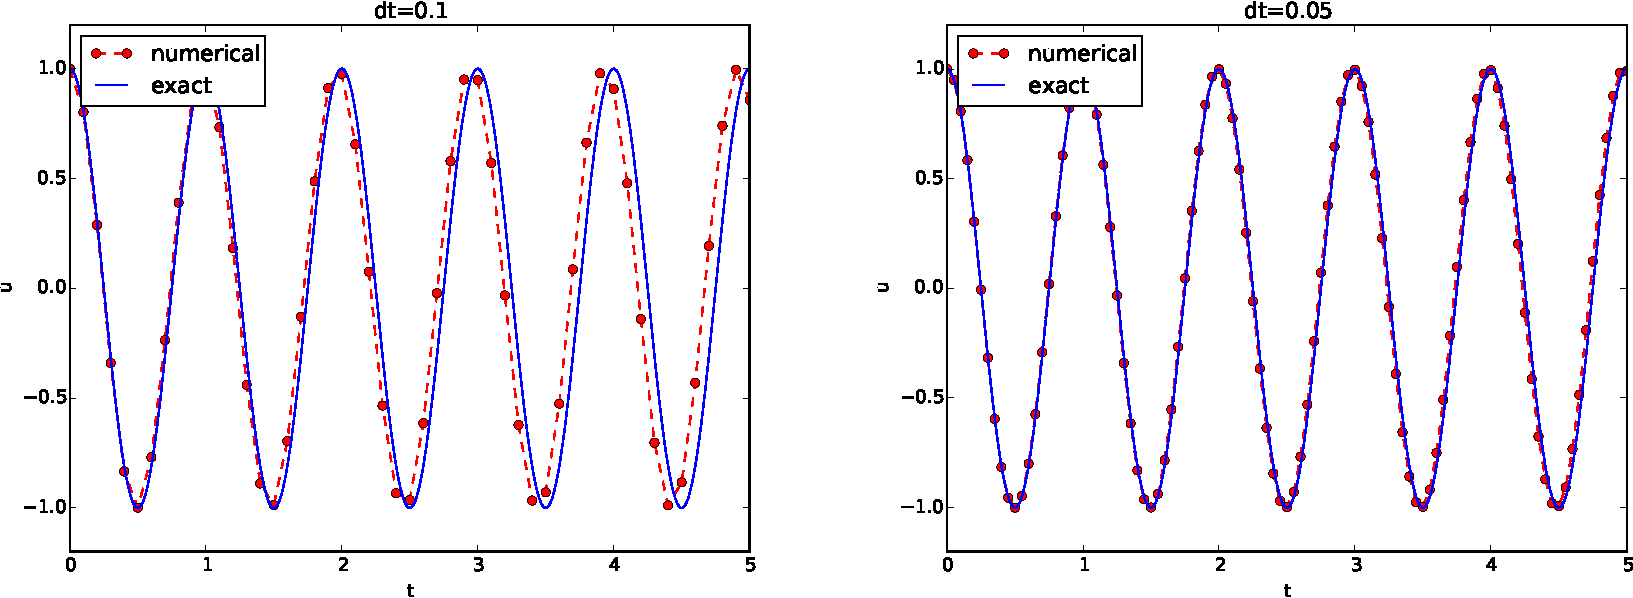
\includegraphics[width=1.0\linewidth]{fig-vib/vib_freq_err1.pdf}}




\begin{itemize}
 \item The numerical solution seems to have right amplitude.

 \item There is an angular frequency error (reduced by reducing the time step).

 \item The total angular frequency error seems to grow with time.
\end{itemize}

\noindent
% !split
\subsection*{Using a moving plot window}

\begin{itemize}
 \item In long time simulations we need a plot window that follows
   the solution.

 \item Method 1: \texttt{scitools.MovingPlotWindow}.

 \item Method 2: \texttt{scitools.avplotter} (ASCII vertical plotter).
\end{itemize}

\noindent
Example:
\begin{cod}{cbg_yellow2}\begin{lstlisting}[language=bash,style=simple,xleftmargin=2mm]
Terminal> python vib_undamped.py --dt 0.05 --num_periods 40
\end{lstlisting}\end{cod}
\noindent

\href{{http://tinyurl.com/opdfafk/pub/mov-vib/vib_undamped_dt0.05/index.html}}{Movie of the moving plot window}.

!splot
\subsection*{Long time simulations visualized with aid of Bokeh: coupled panning of multiple graphs}

\begin{itemize}
 \item \href{{http://bokeh.pydata.org/en/latest/docs/quickstart.html}}{Bokeh} is a
   Python plotting library for fancy web graphics

 \item Example here: long time series with many coupled graphs that can move
   simultaneously
\end{itemize}

\noindent
% inline figure
\centerline{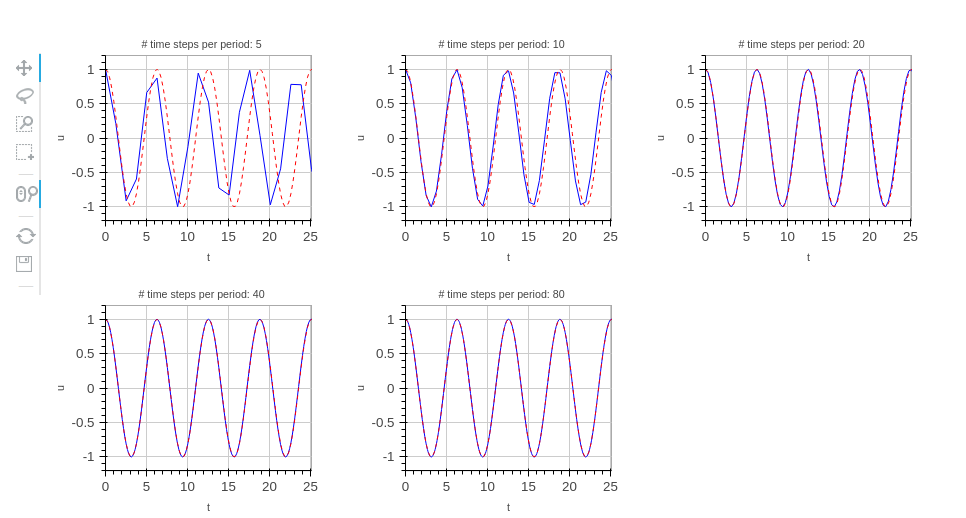
\includegraphics[width=1.0\linewidth]{fig-vib/bokeh_gridplot1.png}}



!splot
\subsection*{How does Bokeh plotting code look like?}

\begin{cod}{cbg_yellow2}\begin{lstlisting}[language=Python,style=simple,xleftmargin=2mm]
def bokeh_plot(u, t, legends, I, w, t_range, filename):
    """
    Make plots for u vs t using the Bokeh library.
    u and t are lists (several experiments can be compared).
    legens contain legend strings for the various u,t pairs.
    """
    if not isinstance(u, (list,tuple)):
        u = [u]  # wrap in list
    if not isinstance(t, (list,tuple)):
        t = [t]  # wrap in list
    if not isinstance(legends, (list,tuple)):
        legends = [legends]  # wrap in list

    import bokeh.plotting as plt
    plt.output_file(filename, mode='cdn', title='Comparison')
    # Assume that all t arrays have the same range
    t_fine = np.linspace(0, t[0][-1], 1001)  # fine mesh for u_e
    tools = 'pan,wheel_zoom,box_zoom,reset,'\ 
            'save,box_select,lasso_select'
    u_range = [-1.2*I, 1.2*I]
    font_size = '8pt'
    p = []  # list of plot objects
    # Make the first figure
    p_ = plt.figure(
        width=300, plot_height=250, title=legends[0],
        x_axis_label='t', y_axis_label='u',
        x_range=t_range, y_range=u_range, tools=tools,
        title_text_font_size=font_size)
    p_.xaxis.axis_label_text_font_size=font_size
    p_.yaxis.axis_label_text_font_size=font_size
    p_.line(t[0], u[0], line_color='blue')
    # Add exact solution
    u_e = u_exact(t_fine, I, w)
    p_.line(t_fine, u_e, line_color='red', line_dash='4 4')
    p.append(p_)
    # Make the rest of the figures and attach their axes to
    # the first figure's axes
    for i in range(1, len(t)):
        p_ = plt.figure(
            width=300, plot_height=250, title=legends[i],
            x_axis_label='t', y_axis_label='u',
            x_range=p[0].x_range, y_range=p[0].y_range, tools=tools,
            title_text_font_size=font_size)
        p_.xaxis.axis_label_text_font_size = font_size
        p_.yaxis.axis_label_text_font_size = font_size
        p_.line(t[i], u[i], line_color='blue')
        p_.line(t_fine, u_e, line_color='red', line_dash='4 4')
        p.append(p_)

    # Arrange all plots in a grid with 3 plots per row
    grid = [[]]
    for i, p_ in enumerate(p):
        grid[-1].append(p_)
        if (i+1) % 3 == 0:
            # New row
            grid.append([])
    plot = plt.gridplot(grid, toolbar_location='left')
    plt.save(plot)
    plt.show(plot)
\end{lstlisting}\end{cod}
\noindent

% !split
\section*{Analysis of the numerical scheme}
\label{vib:model1:analysis}


\begin{center}
\begin{Sbox}
\begin{minipage}{0.85\linewidth}
Can we understand the frequency error?
\end{minipage}
\end{Sbox}
\fbox{\TheSbox}
\end{center}



% inline figure
\centerline{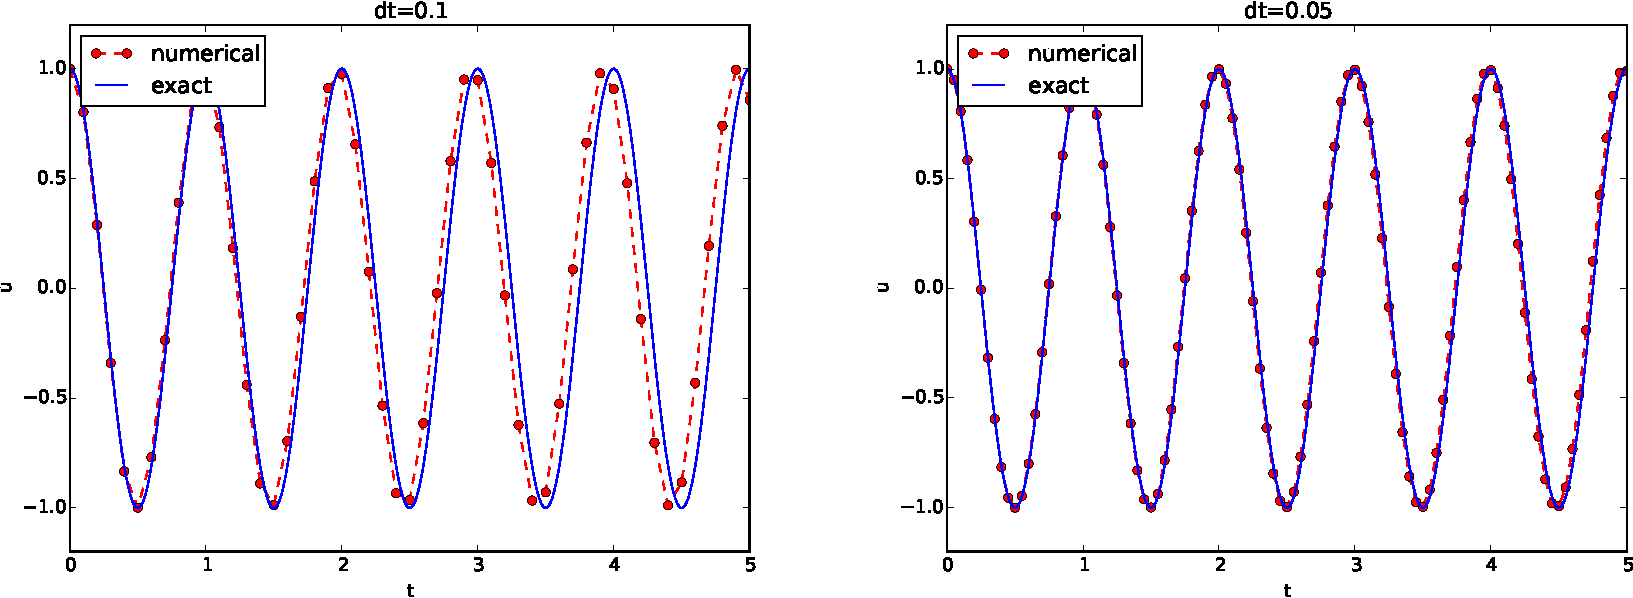
\includegraphics[width=1.0\linewidth]{fig-vib/vib_freq_err1.pdf}}



% !split
\subsection*{Movie of the angular frequency error}

$u^{\prime\prime} + \omega^2 u = 0$, $u(0)=1$, $u^{\prime}(0)=0$,
$\omega=2\pi$, $\uex(t)=\cos (2\pi t)$, $\Delta t = 0.05$ (20 intervals
per period)


\vspace{3mm}




\begin{doconce:movie}
\refstepcounter{doconce:movie:counter}
\begin{center}
% link to external viewer
\href{run:mov-vib/vib_undamped_movie_dt0.05/movie.ogg}{\nolinkurl{mov-vib/vib_undamped_movie_dt0.05/movie.ogg}}
\end{center}
\end{doconce:movie}


% !split
\subsection*{We can derive an exact solution of the discrete equations}

\begin{itemize}
  \item We have a linear, homogeneous, difference equation for $u^n$.

  \item Has solutions $u^n \sim IA^n$, where $A$ is unknown (number).

  \item Here: $\uex(t) =I\cos(\omega t) \sim I\exp{(i\omega t)} = I(e^{i\omega\Delta t})^n$

  \item Trick for simplifying the algebra: $u^n = IA^n$, with $A=\exp{(i\tilde\omega\Delta t)}$, then find $\tilde\omega$

  \item $\tilde\omega$: unknown \emph{numerical frequency} (easier to calculate than $A$)

  \item $\omega - \tilde\omega$ is the angular \emph{frequency error}

  \item Use the real part as the physical relevant part of a complex expression
\end{itemize}

\noindent
% !split
\subsection*{Calculations of an exact solution of the discrete equations}

\[
u^n = IA^n = I\exp{(\tilde\omega \Delta t\, n)}=I\exp{(\tilde\omega t)} =
I\cos (\tilde\omega t) + iI\sin(\tilde \omega t)
\tp
\]

\begin{align*}
[D_tD_t u]^n &= \frac{u^{n+1} - 2u^n + u^{n-1}}{\Delta t^2}\\ 
&= I\frac{A^{n+1} - 2A^n + A^{n-1}}{\Delta t^2}\\ 
&= I\frac{\exp{(i\tilde\omega(t+\Delta t))} - 2\exp{(i\tilde\omega t)} + \exp{(i\tilde\omega(t-\Delta t))}}{\Delta t^2}\\ 
&= I\exp{(i\tilde\omega t)}\frac{1}{\Delta t^2}\left(\exp{(i\tilde\omega(\Delta t))} + \exp{(i\tilde\omega(-\Delta t))} - 2\right)\\ 
&= I\exp{(i\tilde\omega t)}\frac{2}{\Delta t^2}\left(\cosh(i\tilde\omega\Delta t) -1 \right)\\ 
&= I\exp{(i\tilde\omega t)}\frac{2}{\Delta t^2}\left(\cos(\tilde\omega\Delta t) -1 \right)\\ 
&= -I\exp{(i\tilde\omega t)}\frac{4}{\Delta t^2}\sin^2(\frac{\tilde\omega\Delta t}{2})
\end{align*}

% !split
\subsection*{Solving for the numerical frequency}

The scheme
with $u^n=I\exp{(i\omega\tilde\Delta t\, n)}$ inserted gives

\[
-I\exp{(i\tilde\omega t)}\frac{4}{\Delta t^2}\sin^2(\frac{\tilde\omega\Delta t}{2})
+ \omega^2 I\exp{(i\tilde\omega t)} = 0
\]
which after dividing by $I\exp{(i\tilde\omega t)}$ results in
\[
\frac{4}{\Delta t^2}\sin^2(\frac{\tilde\omega\Delta t}{2}) = \omega^2
\]
Solve for $\tilde\omega$:
\[
\tilde\omega = \pm \frac{2}{\Delta t}\sin^{-1}\left(\frac{\omega\Delta t}{2}\right)
\]

\begin{itemize}
 \item Frequency error because $\tilde\omega \neq \omega$.

 \item Note: dimensionless number $p=\omega\Delta t$ is the key parameter \\
   (i.e., no of time intervals per period is important, not $\Delta t$ itself)

 \item But how good is the approximation $\tilde\omega$ to $\omega$?
\end{itemize}

\noindent
% !split
\subsection*{Polynomial approximation of the frequency error}

Taylor series expansion
for small $\Delta t$ gives a formula that is easier to understand:

\begin{cod}{cbg_yellow2}\begin{lstlisting}[language=Python,style=simple,xleftmargin=2mm]
>>> from sympy import *
>>> dt, w = symbols('dt w')
>>> w_tilde = asin(w*dt/2).series(dt, 0, 4)*2/dt
>>> print w_tilde
(dt*w + dt**3*w**3/24 + O(dt**4))/dt  # note the final "/dt"
\end{lstlisting}\end{cod}
\noindent

\[
\tilde\omega = \omega\left( 1 + \frac{1}{24}\omega^2\Delta t^2\right) + {\cal O}(\Delta t^3)
\]
The numerical frequency is too large (to fast oscillations).

% !split
\subsection*{Plot of the frequency error}



% inline figure
\centerline{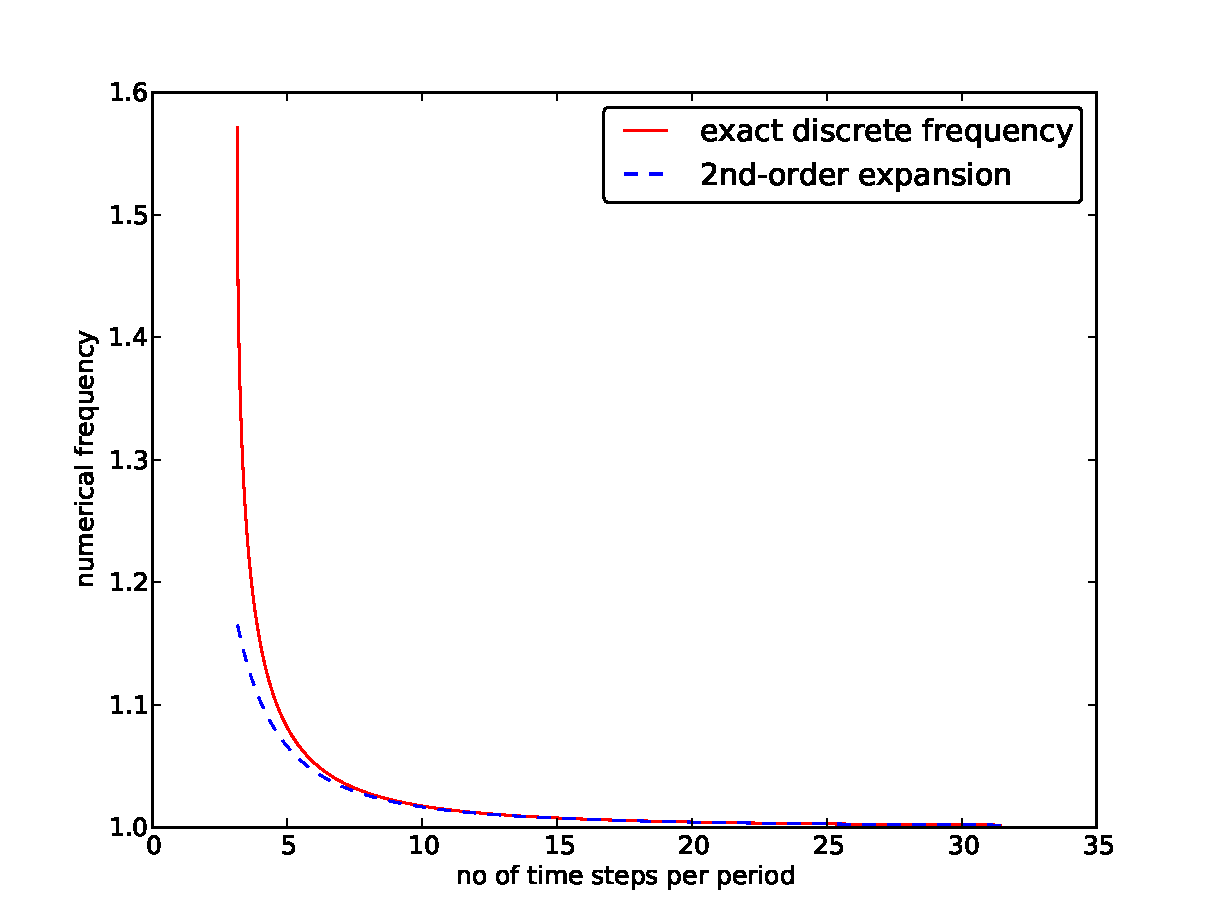
\includegraphics[width=0.9\linewidth]{fig-vib/discrete_freq.pdf}}



Recommendation: 25-30 points per period.


% !split
\subsection*{Exact discrete solution}

\[
u^n = I\cos\left(\tilde\omega n\Delta t\right),\quad
\tilde\omega = \frac{2}{\Delta t}\sin^{-1}\left(\frac{\omega\Delta t}{2}\right)
\]

The error mesh function,

\[ e^n = \uex(t_n) - u^n =
I\cos\left(\omega n\Delta t\right)
- I\cos\left(\tilde\omega n\Delta t\right)
\]
is ideal for verification and further analysis!

\[
e^n = I\cos\left(\omega n\Delta t\right)
- I\cos\left(\tilde\omega n\Delta t\right)
= -2I\sin\left(t\half\left( \omega - \tilde\omega\right)\right)
\sin\left(t\half\left( \omega + \tilde\omega\right)\right)
\]

% !split
\subsection*{Convergence of the numerical scheme}

Can easily show \emph{convergence}:

\[ e^n\rightarrow 0 \hbox{ as }\Delta t\rightarrow 0,\]
because

\[
\lim_{\Delta t\rightarrow 0}
\tilde\omega = \lim_{\Delta t\rightarrow 0}
\frac{2}{\Delta t}\sin^{-1}\left(\frac{\omega\Delta t}{2}\right)
= \omega,
\]
by L'Hopital's rule or simply asking \texttt{sympy}:
or \href{{http://www.wolframalpha.com/input/?i=%282%2Fx%29*asin%28w*x%2F2%29+as+x-%3E0}}{WolframAlpha}:

\begin{cod}{cbg_yellow2}\begin{lstlisting}[language=Python,style=simple,xleftmargin=2mm]
>>> import sympy as sym
>>> dt, w = sym.symbols('x w')
>>> sym.limit((2/dt)*sym.asin(w*dt/2), dt, 0, dir='+')
w
\end{lstlisting}\end{cod}
\noindent



% !split
\subsection*{Stability}

Observations:

\begin{itemize}
 \item Numerical solution has constant amplitude (desired!), but an angular frequency error

 \item Constant amplitude requires $\sin^{-1}(\omega\Delta t/2)$ to be
   real-valued $\Rightarrow |\omega\Delta t/2| \leq 1$

 \item $\sin^{-1}(x)$ is complex if $|x| > 1$, and then $\tilde\omega$ becomes
   complex
\end{itemize}

\noindent
What is the consequence of complex $\tilde\omega$?

\begin{itemize}
 \item Set $\tilde\omega = \tilde\omega_r + i\tilde\omega_i$

 \item Since $\sin^{-1}(x)$ has a \href{{http://www.wolframalpha.com/input/?i=arcsin%28x%29%2C+x+in+%280%2C3%29}}{*negative* imaginary part} for
   $x>1$, $\exp{(i\omega\tilde t)}=\exp{(-\tilde\omega_i t)}\exp{(i\tilde\omega_r t)}$
   leads to exponential growth $e^{-\tilde\omega_it}$
   when $-\tilde\omega_i t > 0$

 \item This is \emph{instability} because the qualitative behavior is wrong
\end{itemize}

\noindent
% !split
\subsection*{The stability criterion}

\index{stability criterion}

Cannot tolerate growth and must therefore demand a \emph{stability criterion}
\[
\frac{\omega\Delta t}{2} \leq 1\quad\Rightarrow\quad
\Delta t \leq \frac{2}{\omega}
\]

Try $\Delta t = \frac{2}{\omega} + 9.01\cdot 10^{-5}$ (\emph{slightly} too big!):



% inline figure
\centerline{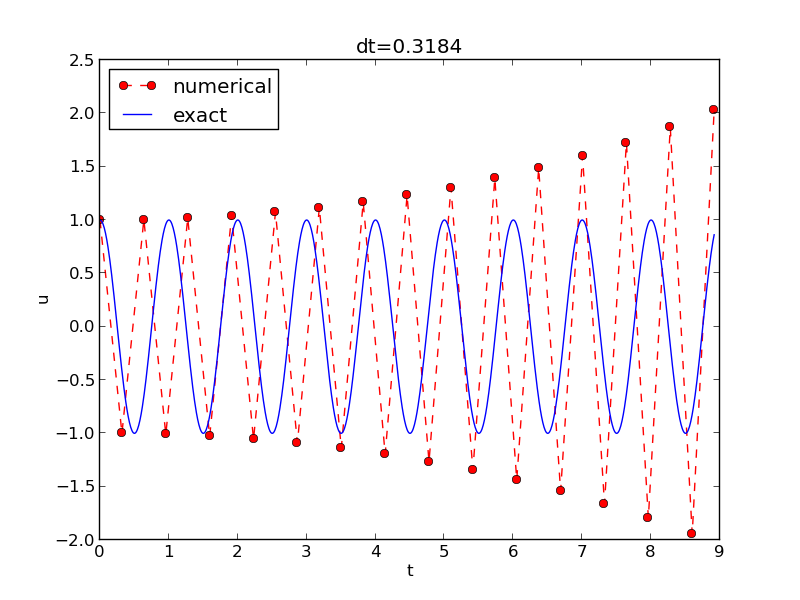
\includegraphics[width=0.8\linewidth]{fig-vib/vib_unstable.png}}



% !split
\subsection*{Summary of the analysis}

We can draw three important conclusions:

\begin{enumerate}
\item The key parameter in the formulas is $p=\omega\Delta t$ (dimensionless)
\begin{enumerate}

  \item Period of oscillations: $P=2\pi/\omega$

  \item Number of time steps per period: $N_P=P/\Delta t$

  \item $\Rightarrow\ p=\omega\Delta t = 2\pi/ N_P \sim 1/N_P$

  \item The smallest possible $N_P$ is 2 $\Rightarrow$ $p\in (0,\pi]$

\end{enumerate}

\noindent
\item For $p\leq 2$ the amplitude of $u^n$ is constant (stable solution)

\item $u^n$ has a relative frequency error
   $\tilde\omega/\omega \approx 1 + \frac{1}{24}p^2$, making numerical
   peaks occur too early
\end{enumerate}

\noindent
% !split
\section*{Alternative schemes based on 1st-order equations}
\label{vib:model2x2}

% !split
\subsection*{Rewriting 2nd-order ODE as system of two 1st-order ODEs}

The vast collection of ODE solvers (e.g., in \href{{https://github.com/hplgit/odespy}}{Odespy}) cannot be applied to
\[ u^{\prime\prime} + \omega^2 u = 0\]
unless we write this higher-order ODE as a system of 1st-order ODEs.

Introduce an auxiliary variable $v=u^{\prime}$:

\begin{align}
u^{\prime} &= v,
\label{vib:model2x2:ueq}\\ 
v^{\prime} &= -\omega^2 u
\label{vib:model2x2:veq}
\tp
\end{align}

Initial conditions: $u(0)=I$ and $v(0)=0$.

% !split
\subsection*{The Forward Euler scheme}

We apply the Forward Euler scheme to each component equation:

\begin{align*}
[D_t^+ u &= v]^n,\\ 
[D_t^+ v &= -\omega^2 u]^n,
\end{align*}
or written out,

\begin{align}
u^{n+1} &= u^n + \Delta t v^n,\\ 
v^{n+1} &= v^n -\Delta t \omega^2 u^n
\tp
\end{align}

% !split
\subsection*{The Backward Euler scheme}

We apply the Backward Euler scheme to each component equation:

\begin{align}
 [D_t^- u &= v]^{n+1},\\ 
 [D_t^- v &= -\omega u]^{n+1} \tp
\end{align}
Written out:
\begin{align}
u^{n+1} - \Delta t v^{n+1} = u^{n},\\ 
v^{n+1} + \Delta t \omega^2 u^{n+1} = v^{n}
\tp
\end{align}
This is a \emph{coupled} $2\times 2$ system for the new values at $t=t_{n+1}$!

% !split
\subsection*{The Crank-Nicolson scheme}

\begin{align}
[D_t u &= \overline{v}^t]^{n+\half},\\ 
[D_t v &= -\omega \overline{u}^t]^{n+\half}
\tp
\end{align}
The result is also a coupled system:

\begin{align}
u^{n+1} - \half\Delta t v^{n+1} &= u^{n} + \half\Delta t v^{n},\\ 
v^{n+1} + \half\Delta t \omega^2 u^{n+1} &= v^{n}
- \half\Delta t \omega^2 u^{n}
\tp
\end{align}

% !split
\subsection*{Comparison of schemes via Odespy}

Can use
\href{{https://github.com/hplgit/odespy}}{Odespy} to compare many methods
for first-order schemes:

\begin{cod}{cbg_yellow2}\begin{lstlisting}[language=Python,style=simple,xleftmargin=2mm]
import odespy
import numpy as np

def f(u, t, w=1):
    u, v = u  # u is array of length 2 holding our [u, v]
    return [v, -w**2*u]

def run_solvers_and_plot(solvers, timesteps_per_period=20,
                         num_periods=1, I=1, w=2*np.pi):
    P = 2*np.pi/w  # duration of one period
    dt = P/timesteps_per_period
    Nt = num_periods*timesteps_per_period
    T = Nt*dt
    t_mesh = np.linspace(0, T, Nt+1)

    legends = []
    for solver in solvers:
        solver.set(f_kwargs={'w': w})
        solver.set_initial_condition([I, 0])
        u, t = solver.solve(t_mesh)
\end{lstlisting}\end{cod}
\noindent

% !split
\subsection*{Forward and Backward Euler and Crank-Nicolson}

\begin{cod}{cbg_yellow2}\begin{lstlisting}[language=Python,style=simple,xleftmargin=2mm]
solvers = [
    odespy.ForwardEuler(f),
    # Implicit methods must use Newton solver to converge
    odespy.BackwardEuler(f, nonlinear_solver='Newton'),
    odespy.CrankNicolson(f, nonlinear_solver='Newton'),
    ]
\end{lstlisting}\end{cod}
\noindent

Two plot types:

\begin{itemize}
  \item $u(t)$ vs $t$

  \item Parameterized curve $(u(t), v(t))$ in \emph{phase space}

  \item Exact curve is an ellipse: $(I\cos\omega t, -\omega I\sin\omega t)$,
    closed and periodic
\end{itemize}

\noindent
% !split
\subsection*{Phase plane plot of the numerical solutions}



% inline figure
\centerline{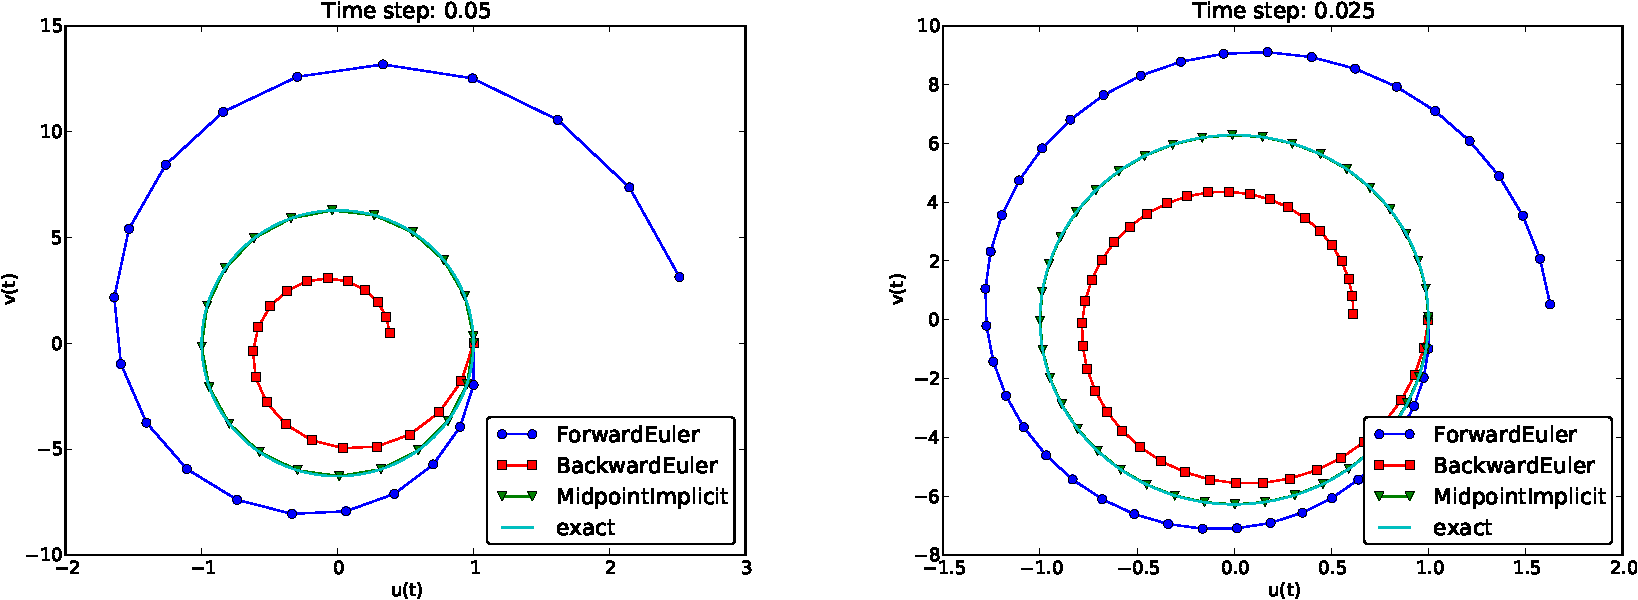
\includegraphics[width=1.0\linewidth]{fig-vib/vib_theta_1_pp.pdf}}



Note: CrankNicolson in Odespy leads to the name MidpointImplicit in plots.

% !split
\subsection*{Plain solution curves}


\begin{figure}[!ht]  % vib:model1:1st:odespy:theta
  \centerline{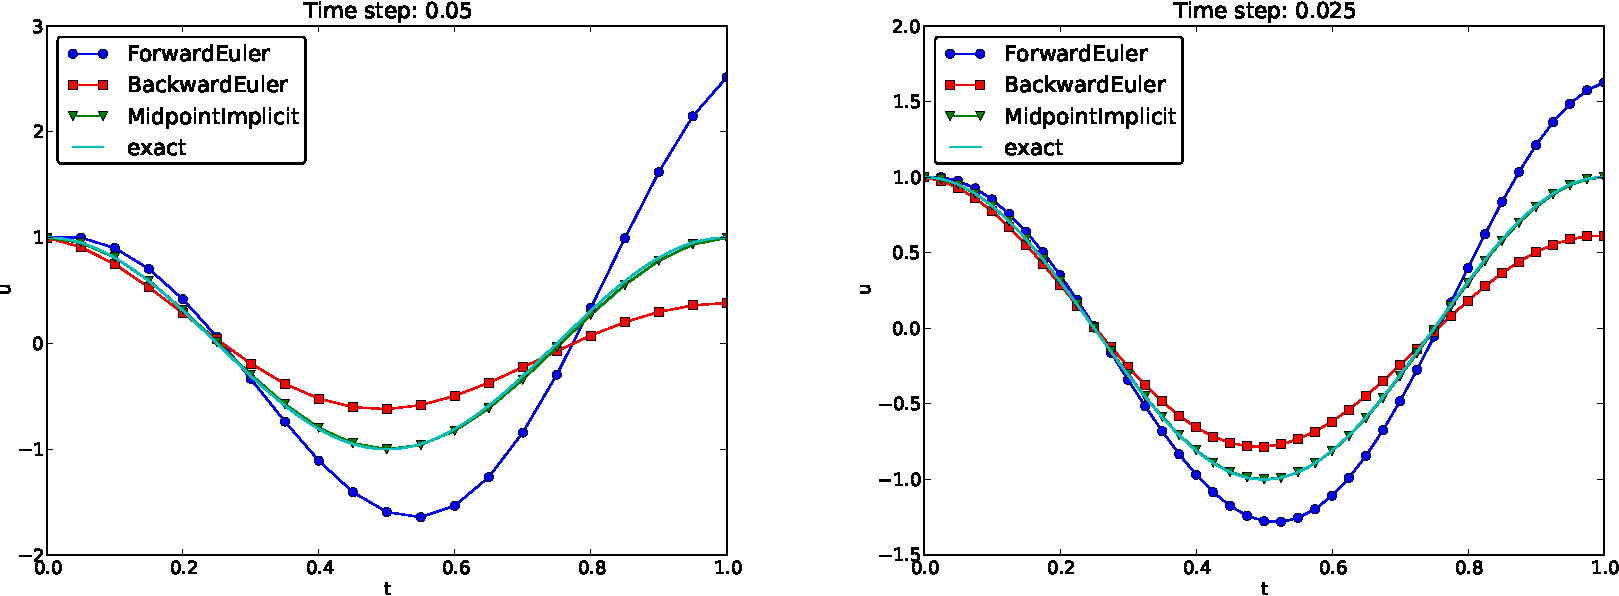
\includegraphics[width=1.0\linewidth]{fig-vib/vib_theta_1_u.pdf}}
  \caption{
  Comparison of classical schemes. \label{vib:model1:1st:odespy:theta}
  }
\end{figure}
%\clearpage % flush figures vib:model1:1st:odespy:theta


% !split
\subsection*{Observations from the figures}

\begin{itemize}
  \item Forward Euler has growing amplitude and outward $(u,v)$ spiral - pumps
    energy into the system.

  \item Backward Euler is opposite: decreasing amplitude, inward sprial,
    extracts energy.

  \item \textbf{Forward and Backward Euler are useless for vibrations.}

  \item Crank-Nicolson (MidpointImplicit) looks much better.
\end{itemize}

\noindent
% !split
\subsection*{Runge-Kutta methods of order 2 and 4; short time series}



% inline figure
\centerline{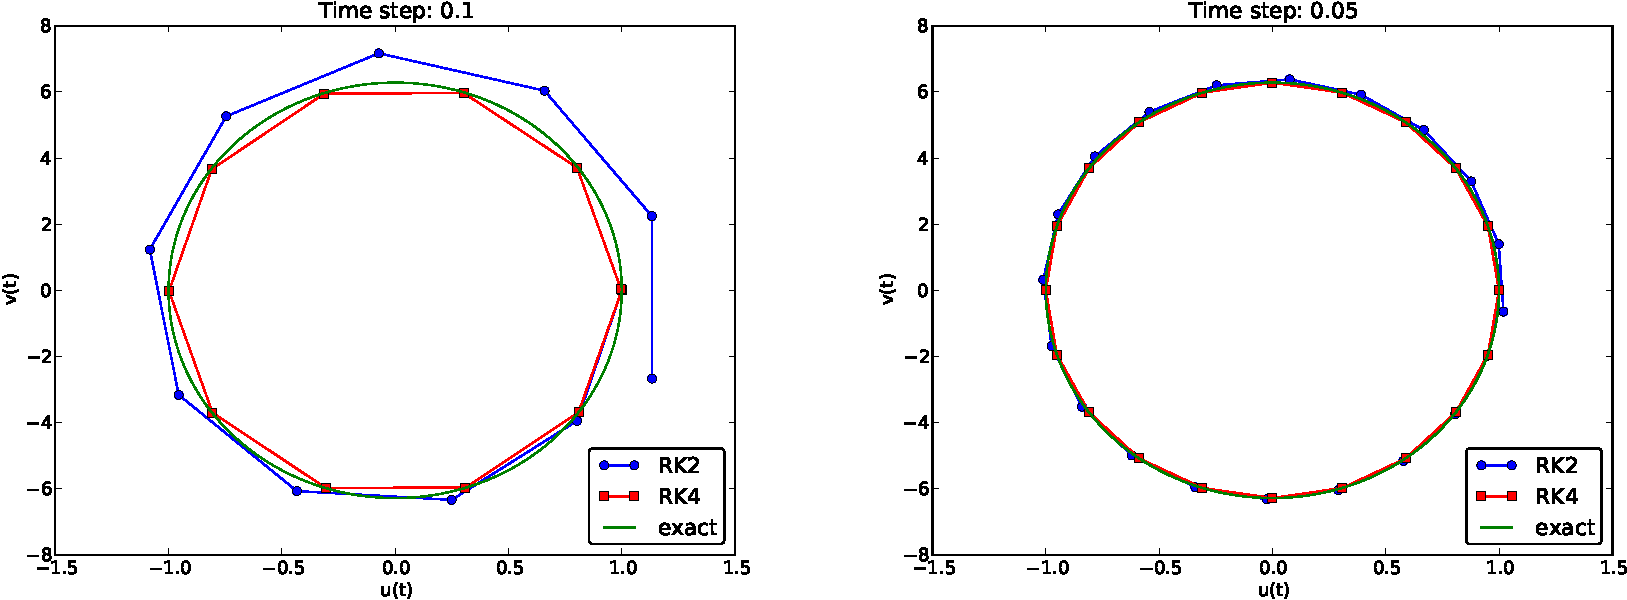
\includegraphics[width=1.0\linewidth]{fig-vib/vib_RK_1_pp.pdf}}





% inline figure
\centerline{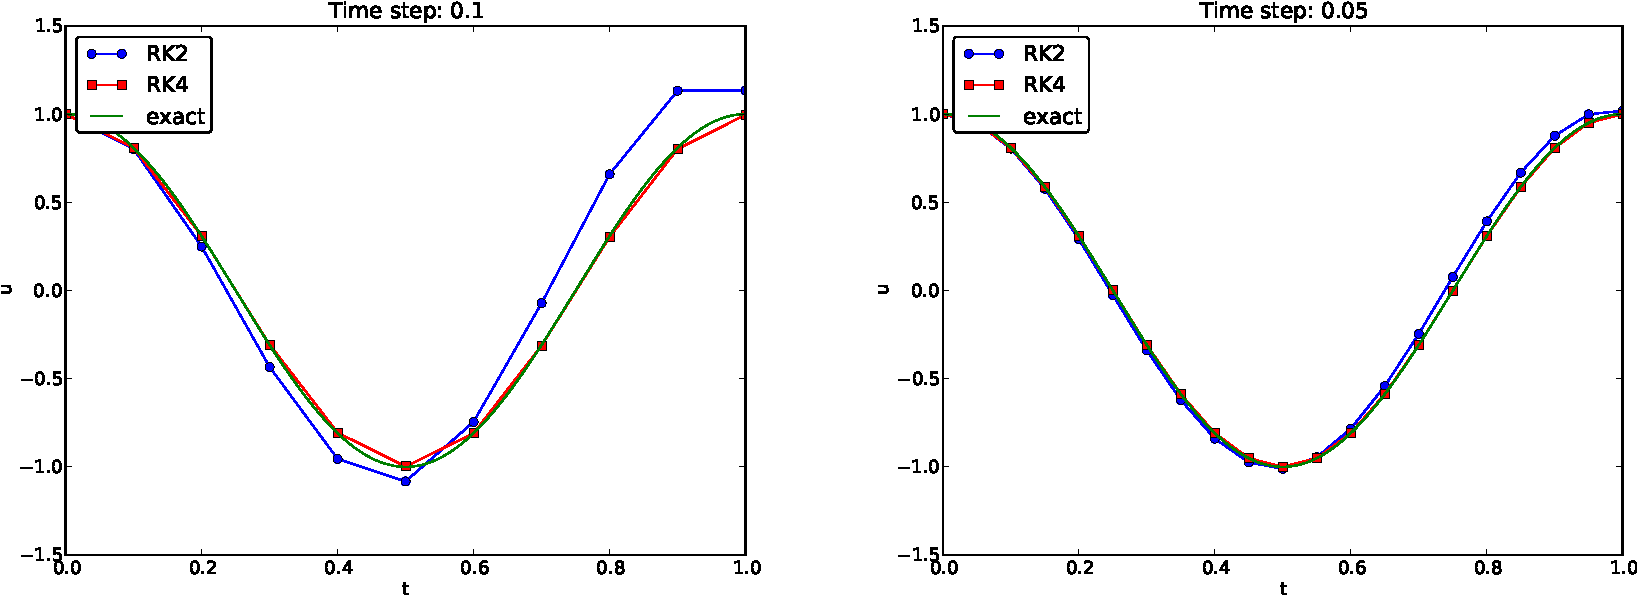
\includegraphics[width=1.0\linewidth]{fig-vib/vib_RK_1_u.pdf}}



% !split
\subsection*{Runge-Kutta methods of order 2 and 4; longer time series}



% inline figure
\centerline{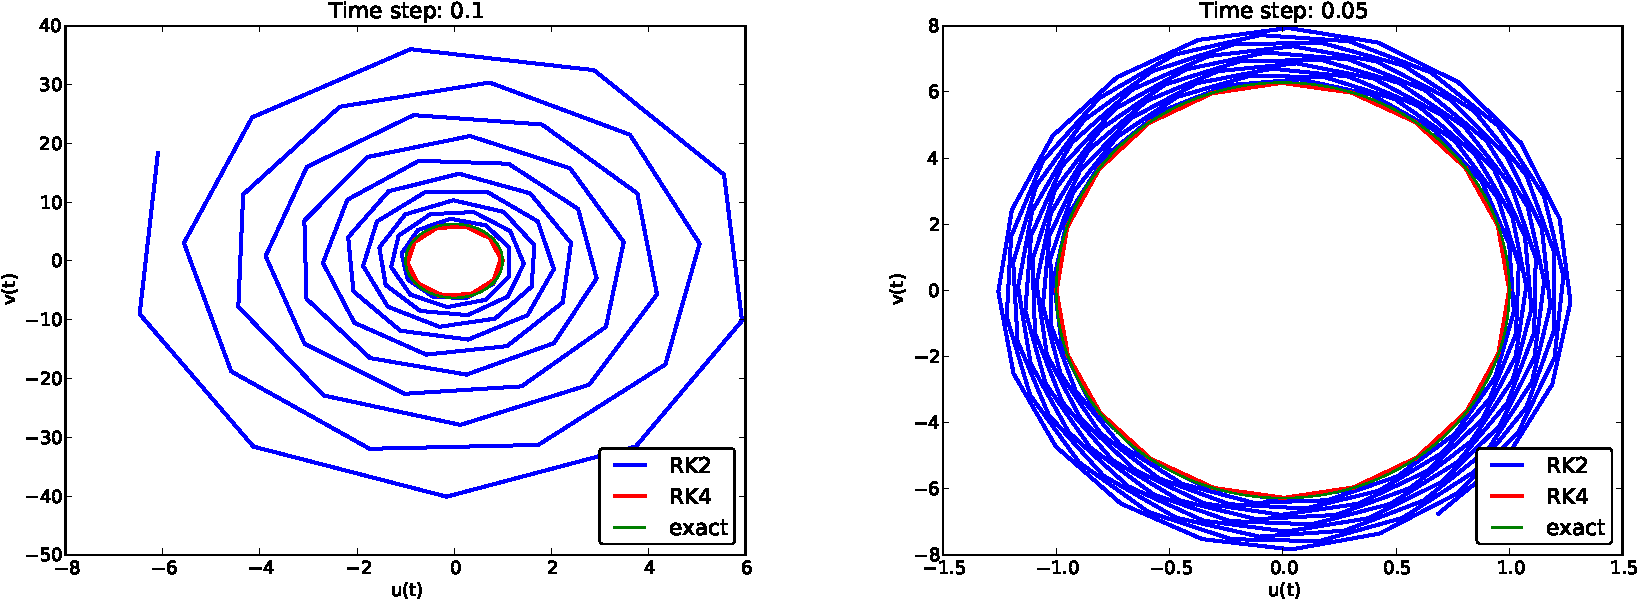
\includegraphics[width=1.0\linewidth]{fig-vib/vib_RK_10_pp.pdf}}





% inline figure
\centerline{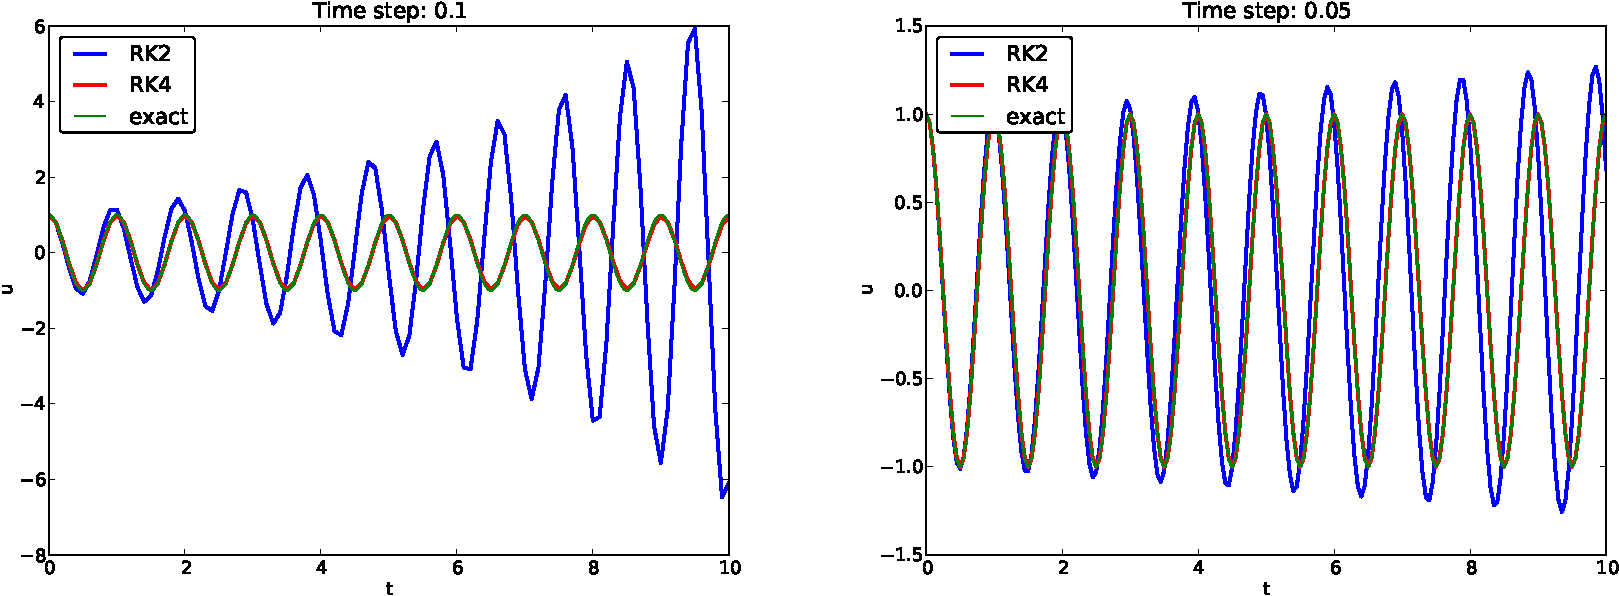
\includegraphics[width=1.0\linewidth]{fig-vib/vib_RK_10_u.pdf}}



% !split
\subsection*{Crank-Nicolson; longer time series}



% inline figure
\centerline{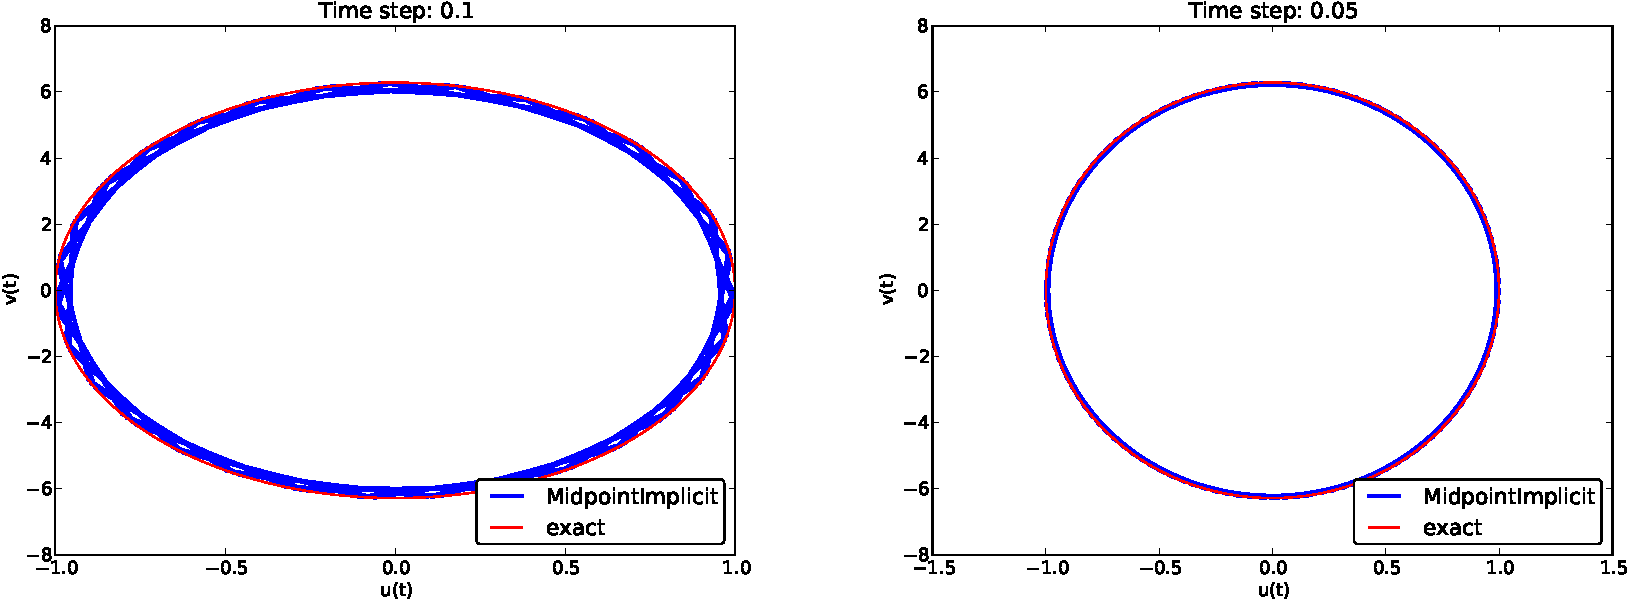
\includegraphics[width=1.0\linewidth]{fig-vib/vib_CN_10_pp.pdf}}





% inline figure
\centerline{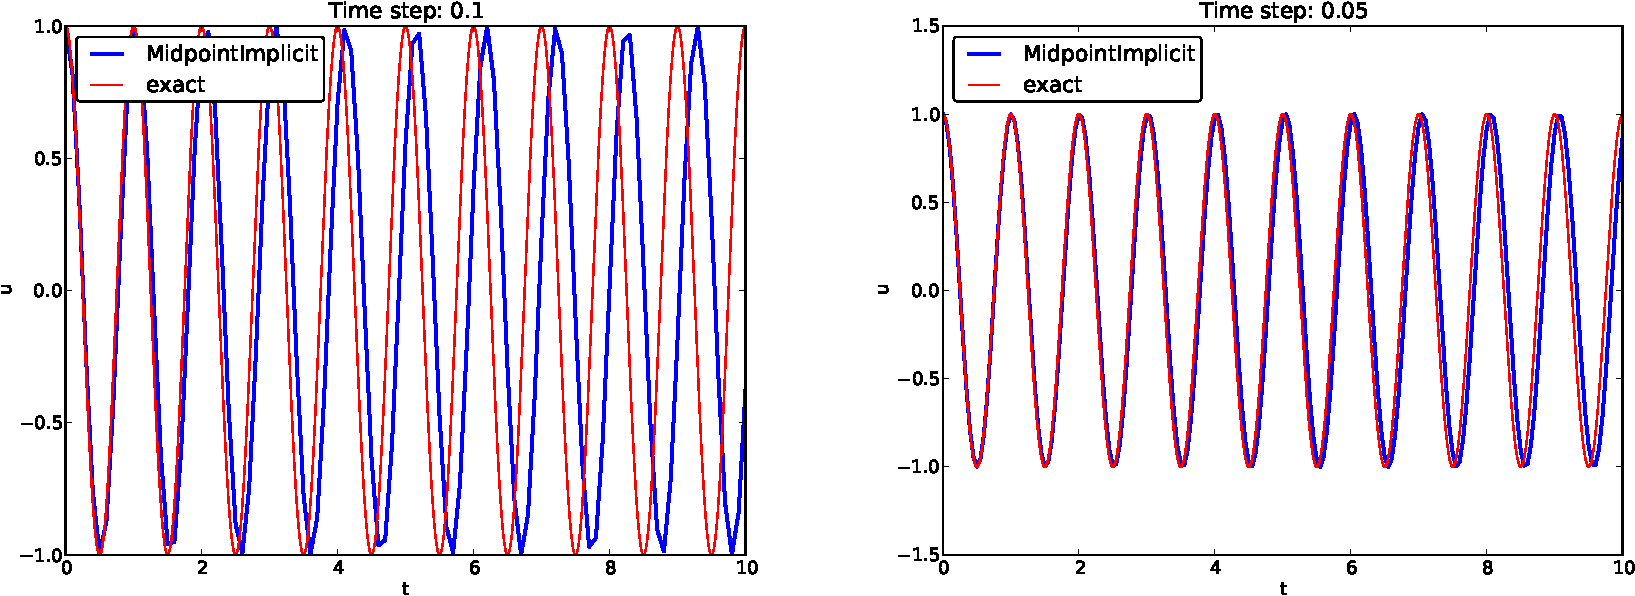
\includegraphics[width=1.0\linewidth]{fig-vib/vib_CN_10_u.pdf}}



(MidpointImplicit means CrankNicolson in Odespy)

% !split
\subsection*{Observations of RK and CN methods}

\begin{itemize}
  \item 4th-order Runge-Kutta is very accurate, also for large $\Delta t$.

  \item 2th-order Runge-Kutta is almost as bad as Forward and Backward
    Euler.

  \item Crank-Nicolson is accurate, but the amplitude is not as accurate
    as the difference scheme for $u^{\prime\prime}+\omega^2u=0$.
\end{itemize}

\noindent
% !split
\subsection*{Energy conservation property}

The model

\[ u^{\prime\prime} + \omega^2 u = 0,\quad u(0)=I,\ u^{\prime}(0)=V,\]
has the nice \emph{energy conservation property} that

\[ E(t) = \half(u^{\prime})^2 + \half\omega^2u^2 = \hbox{const}\tp\]
This can be used to check solutions.

% !split
\subsection*{Derivation of the energy conservation property}

Multiply $u^{\prime\prime}+\omega^2u=0$ by $u^{\prime}$ and integrate:

\[ \int_0^T u^{\prime\prime}u^{\prime} dt + \int_0^T\omega^2 u u^{\prime} dt = 0\tp\]
Observing that

\[ u^{\prime\prime}u^{\prime} = \frac{d}{dt}\half(u^{\prime})^2,\quad uu^{\prime} = \frac{d}{dt} {\half}u^2,\]
we get

\[
\int_0^T (\frac{d}{dt}\half(u^{\prime})^2 + \frac{d}{dt} \half\omega^2u^2)dt = E(T) - E(0),
\]
where

\[
E(t) = \half(u^{\prime})^2 + \half\omega^2u^2
\]

% !split
\subsection*{Remark about $E(t)$}

$E(t)$ does not measure energy, energy per mass unit.

Starting with an ODE coming directly from Newton's 2nd law $F=ma$ with
a spring force $F=-ku$ and $ma=mu^{\prime\prime}$ ($a$: acceleration, $u$: displacement),
we have

\[ mu^{\prime\prime} + ku = 0\]
Integrating this equation gives a physical energy balance:

\[
E(t) = \underbrace{{\half}mv^2}_{\hbox{kinetic energy} }
+ \underbrace{{\half}ku^2}_{\hbox{potential energy}} = E(0),\quad v=u^{\prime}
\]
Note: the balance is not valid if we add other terms to the ODE.


% !split
\subsection*{The Euler-Cromer method; idea}
\label{vib:model2x2:EulerCromer}

2x2 system for $u^{\prime\prime}+\omega^2u=0$:

\begin{align*}
v^{\prime} &= -\omega^2u\\ 
u^{\prime} &= v
\end{align*}

Forward-backward discretization:

\begin{itemize}
  \item Update $v$ with Forward Euler

  \item Update $u$ with Backward Euler, using latest $v$
\end{itemize}

\noindent
\begin{align}
[D_t^+v &= -\omega^2u]^n\\ 
[D_t^-u &= v]^{n+1}
\end{align}

% !split
\subsection*{The Euler-Cromer method; complete formulas}

Written out:

\begin{align}
u^0 &= I,\\ 
v^0 &= 0,\\ 
v^{n+1} &= v^n -\Delta t \omega^2u^{n}
\label{vib:model2x2:EulerCromer:veq1}\\ 
u^{n+1} &= u^n + \Delta t v^{n+1}
\label{vib:model2x2:EulerCromer:ueq1}
\end{align}

Names: Forward-backward scheme, \href{{http://en.wikipedia.org/wiki/Semi-implicit_Euler_method}}{Semi-implicit Euler method}, symplectic
Euler, semi-explicit Euler, Newton-Stormer-Verlet, and \emph{Euler-Cromer}.

% !split
\subsection*{Euler-Cromer is equivalent to the scheme for $u^{\prime\prime}+\omega^2u=0$}

\begin{itemize}
 \item Forward Euler and Backward Euler have error $\Oof{\Delta t}$

 \item What about the overall scheme? Expect $\Oof{\Delta t}$...
\end{itemize}

\noindent
We can eliminate $v^n$ and $v^{n+1}$, resulting in

\[
u^{n+1} = 2u^n - u^{n-1} - \Delta t^2 \omega^2u^{n}
\]

which is the centered finite differrence scheme for $u^{\prime\prime}+\omega^2u=0$!

% !split
\subsection*{The schemes are not equivalent wrt the initial conditions}

\[ u^{\prime}=v=0\quad\Rightarrow\quad v^0=0,\]
so

\begin{align*}
v^1 &= v^0 - \Delta t\omega^2 u^0 = - \Delta t\omega^2 u^0\\ 
u^1 &= u^0 + \Delta t v^1 = u^0 - \Delta t\omega^2 u^0 !=
\underbrace{u^0 - \frac{1}{2}\Delta t\omega^2 u^0}_{\mbox{from }[D_tD_t u +\omega^2 u=0]^n\mbox{ and }[D_{2t}u=0]^0}
\end{align*}

The exact discrete solution derived earlier does not fit the Euler-Cromer
scheme because of mismatch for $u^1$.

% !split
\section*{Generalization: damping, nonlinear spring, and external excitation}
\label{vib:model2}

\[
mu'' + f(u') + s(u) = F(t),\quad u(0)=I,\ u'(0)=V,\ t\in (0,T]
\]
Input data: $m$, $f(u')$, $s(u)$, $F(t)$, $I$, $V$, and $T$.

Typical choices of $f$ and $s$:

\begin{itemize}
 \item linear damping $f(u')=bu$, or

 \item quadratic damping $f(u')=bu'|u'|$

 \item linear spring $s(u)=cu$

 \item nonlinear spring $s(u)\sim \sin(u)$ (pendulum)
\end{itemize}

\noindent
% !split
\subsection*{A centered scheme for linear damping}
\label{vib:ode2:fdm:flin}

\[
[mD_tD_t u + f(D_{2t}u) + s(u) = F]^n
\]
Written out

\[
m\frac{u^{n+1}-2u^n + u^{n-1}}{\Delta t^2}
+ f(\frac{u^{n+1}-u^{n-1}}{2\Delta t}) + s(u^n) = F^n
\]
Assume $f(u')$ is linear in $u'=v$:

\[
u^{n+1} = \left(2mu^n + (\frac{b}{2}\Delta t - m)u^{n-1} +
\Delta t^2(F^n - s(u^n))
\right)(m + \frac{b}{2}\Delta t)^{-1}
\]

% !split
\subsection*{Initial conditions}

$u(0)=I$, $u'(0)=V$:

\begin{align*}
\lbrack u &=I\rbrack^0\quad\Rightarrow\quad u^0=I\\ 
\lbrack D_{2t}u &=V\rbrack^0\quad\Rightarrow\quad u^{-1} = u^{1} - 2\Delta t V
\end{align*}
End result:

\[
u^1 = u^0 + \Delta t\, V
+ \frac{\Delta t^2}{2m}(-bV - s(u^0) + F^0)
\]
Same formula for $u^1$ as when using a centered scheme for $u''+\omega u=0$.

% !split
\subsection*{Linearization via a geometric mean approximation}
\label{vib:ode2:fdm:fquad}

\begin{itemize}
 \item $f(u')=bu'|u'|$ leads to a quadratic equation for $u^{n+1}$

 \item Instead of solving the quadratic equation, we use a geometric mean
   approximation
\end{itemize}

\noindent
In general, the geometric mean approximation reads
\[ (w^2)^n \approx w^{n-\half}w^{n+\half}\tp\]
For $|u'|u'$ at $t_n$:

\[ [u'|u'|]^n \approx u'(t_n+{\half})|u'(t_n-{\half})|\tp\]
For $u'$ at $t_{n\pm 1/2}$ we use centered difference:

\[
u'(t_{n+1/2})\approx [D_t u]^{n+\half},\quad u'(t_{n-1/2})\approx [D_t u]^{n-\half}
\]

% !split
\subsection*{A centered scheme for quadratic damping}

After some algebra:

\begin{align*}
u^{n+1} &=  \left( m + b|u^n-u^{n-1}|\right)^{-1}\times \\ 
& \qquad \left(2m u^n - mu^{n-1} + bu^n|u^n-u^{n-1}| + \Delta t^2 (F^n - s(u^n))
\right)
\end{align*}

% !split
\subsection*{Initial condition for quadratic damping}

Simply use that $u'=V$ in the scheme when $t=0$ ($n=0$):

\[
[mD_tD_t u + bV|V| + s(u) = F]^0
\]

which gives

\[
u^1 = u^0 + \Delta t V + \frac{\Delta t^2}{2m}\left(-bV|V| - s(u^0) + F^0\right)
\]

% !split
\subsection*{Algorithm}

\begin{enumerate}
 \item $u^0=I$

 \item compute $u^1$ (formula depends on linear/quadratic damping)

 \item for $n=1,2,\ldots,N_t-1$:
\begin{enumerate}

   \item compute $u^{n+1}$ from formula (depends on linear/quadratic damping)
\end{enumerate}

\noindent
\end{enumerate}

\noindent
% !split
\subsection*{Implementation}

\begin{cod}{cbg_yellow2}\begin{lstlisting}[language=Python,style=simple,xleftmargin=2mm]
def solver(I, V, m, b, s, F, dt, T, damping='linear'):
    dt = float(dt); b = float(b); m = float(m) # avoid integer div.
    Nt = int(round(T/dt))
    u = zeros(Nt+1)
    t = linspace(0, Nt*dt, Nt+1)

    u[0] = I
    if damping == 'linear':
        u[1] = u[0] + dt*V + dt**2/(2*m)*(-b*V - s(u[0]) + F(t[0]))
    elif damping == 'quadratic':
        u[1] = u[0] + dt*V + \ 
               dt**2/(2*m)*(-b*V*abs(V) - s(u[0]) + F(t[0]))

    for n in range(1, Nt):
        if damping == 'linear':
            u[n+1] = (2*m*u[n] + (b*dt/2 - m)*u[n-1] +
                      dt**2*(F(t[n]) - s(u[n])))/(m + b*dt/2)
        elif damping == 'quadratic':
            u[n+1] = (2*m*u[n] - m*u[n-1] + b*u[n]*abs(u[n] - u[n-1])
                      + dt**2*(F(t[n]) - s(u[n])))/\ 
                      (m + b*abs(u[n] - u[n-1]))
    return u, t
\end{lstlisting}\end{cod}
\noindent


% !split
\subsection*{Verification}
\label{vib:ode2:verify}

\begin{itemize}
 \item Constant solution $\uex = I$ ($V=0$) fulfills the ODE problem
   and the discrete equations. Ideal for debugging!

 \item Linear solution $\uex = Vt+I$ fulfills the ODE problem and
   the discrete equations.

 \item Quadratic solution $\uex = bt^2 + Vt + I$ fulfills the ODE
   problem and the discrete equations with linear damping, but not
   for quadratic damping.
   A special discrete source term can allow $\uex$ to also fulfill
   the discrete equations with quadratic damping.
\end{itemize}

\noindent
% !split
\subsection*{Demo program}

\href{{http://tinyurl.com/nm5587k/vib/vib.py}}{\nolinkurl{vib.py}} supports input via the command line:

\begin{cod}{cbg_yellow2}\begin{lstlisting}[language=bash,style=simple,xleftmargin=2mm]
Terminal> python vib.py --s 'sin(u)' --F '3*cos(4*t)' --c 0.03
\end{lstlisting}\end{cod}
\noindent
This results in a \href{{http://tinyurl.com/opdfafk/pub/mov-vib/vib_generalized_dt0.05/index.html}}{moving window following the function} on the screen.



% inline figure
\centerline{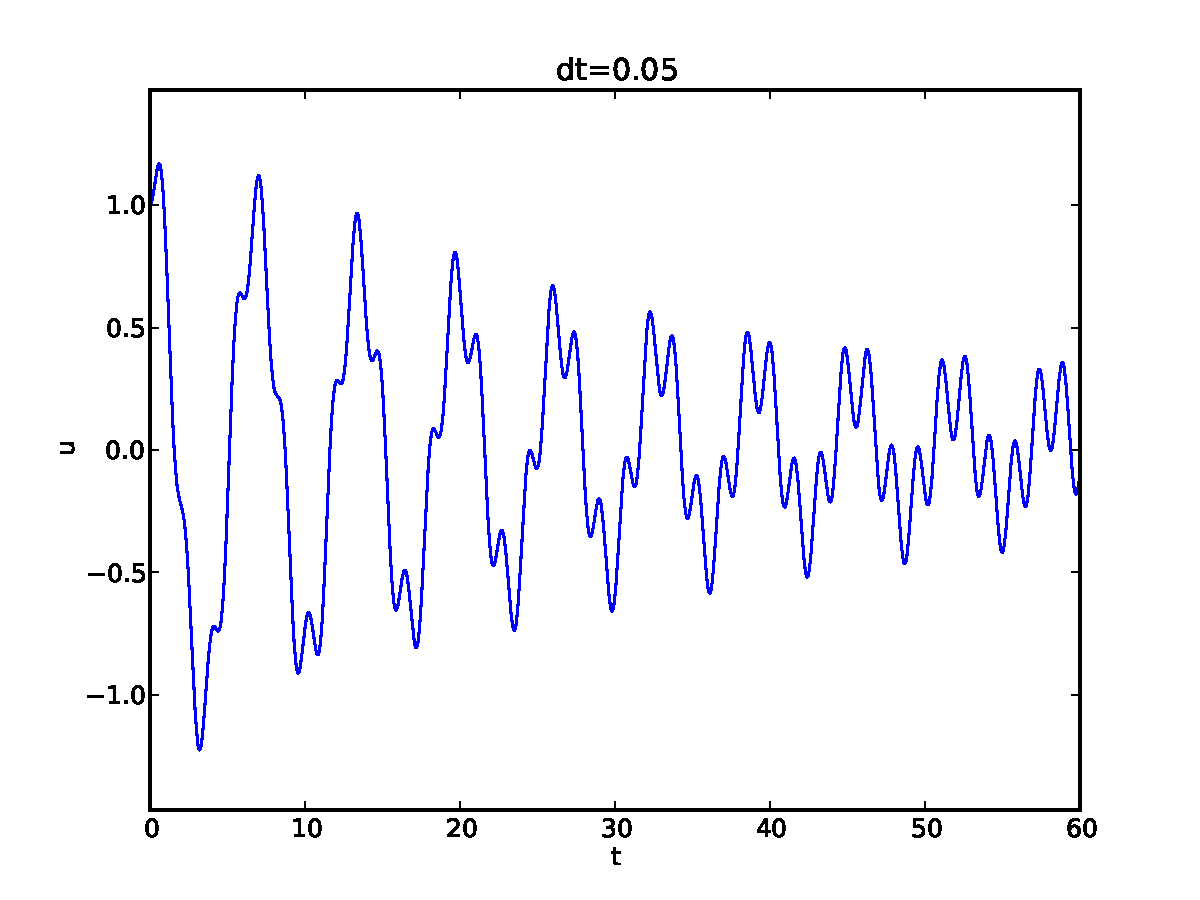
\includegraphics[width=0.9\linewidth]{fig-vib/vib_gen_demo.pdf}}



% !split
\subsection*{Euler-Cromer formulation}

We rewrite

\[
mu'' + f(u') + s(u) = F(t),\quad u(0)=I,\ u'(0)=V,\ t\in (0,T]
\]
as a first-order ODE system

\begin{align*}
u' &= v
\\ 
v' &= m^{-1}\left(F(t) - f(v) - s(u)\right)
\end{align*}

% !split
\subsection*{Staggered grid}

\begin{itemize}
 \item $u$ is unknown at $t_n$: $u^n$

 \item $v$ is unknown at $t_{n+1/2}$: $v^{n+\half}$

 \item All derivatives are approximated by centered differences
\end{itemize}

\noindent
\begin{align*}
\lbrack D_t u &= v\rbrack^{n-\half}
\\ 
\lbrack D_tv &= m^{-1}\left(F(t) - f(v) - s(u)\right)\rbrack^n
\end{align*}

Written out,

\begin{align*}
\frac{u^n - u^{n-1}}{\Delta t} &= v^{n-\half}\\ 
\frac{v^{n+\half} - v^{n-\half}}{\Delta t}
&= m^{-1}\left(F^n - f(v^n) - s(u^n)\right)
\end{align*}

Problem: $f(v^n)$

% !split
\subsection*{Linear damping}

With $f(v)=bv$, we can use an arithmetic mean for $bv^n$ a la
Crank-Nicolson schemes.

\begin{align*}
u^n & = u^{n-1} + {\Delta t}v^{n-\half},\\ 
v^{n+\half} &= \left(1 + \frac{b}{2m}\Delta t\right)^{-1}\left(
v^{n-\half} + {\Delta t}
m^{-1}\left(F^n - {\half}f(v^{n-\half}) - s(u^n)\right)\right)\tp
\end{align*}

% !split
\subsection*{Quadratic damping}

With $f(v)=b|v|v$, we can use a geometric mean

\[
b|v^n|v^n\approx b|v^{n-\half}|v^{n+\half},
\]
resulting in

\begin{align*}
u^n & = u^{n-1} + {\Delta t}v^{n-\half},\\ 
v^{n+\half} &= (1 + \frac{b}{m}|v^{n-\half}|\Delta t)^{-1}\left(
v^{n-\half} + {\Delta t}
m^{-1}\left(F^n - s(u^n)\right)\right)\tp
\end{align*}

% !split
\subsection*{Initial conditions}

\begin{align*}
u^0 &= I\\ 
v^{\half} &= V - \half\Delta t\omega^2I
\end{align*}

% ------------------- end of main content ---------------

% #ifdef PREAMBLE
\cleardoublepage\phantomsection  % trick to get correct link to Index
\printindex

\end{document}
% #endif

